\documentclass[tikz,border=5pt]{standalone}
\begin{document}
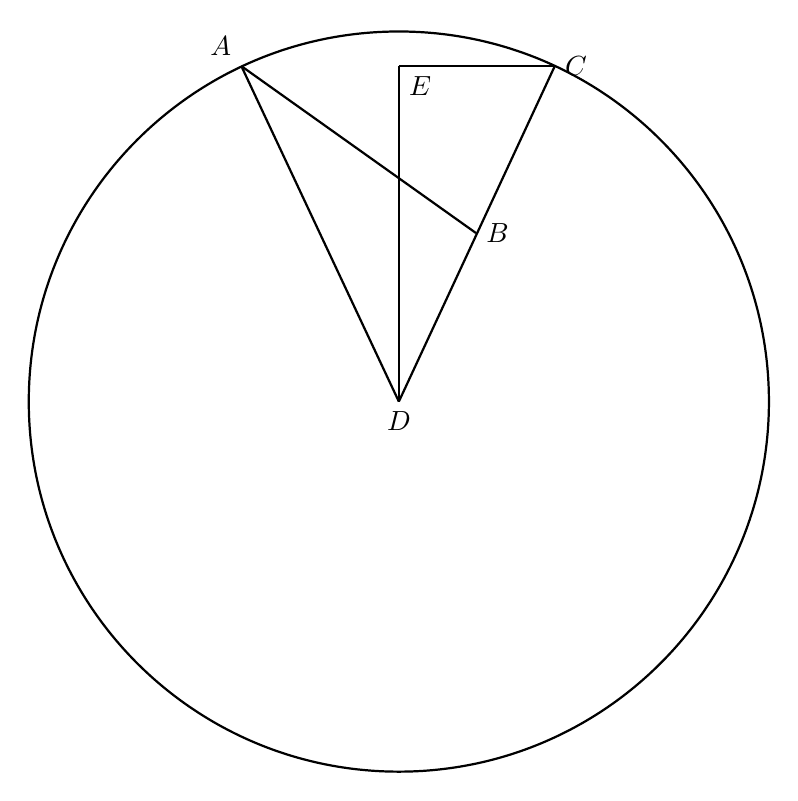
\begin{tikzpicture}[line width=0.8pt]
  % Circle centered at D
  \draw (0,0) circle (4.7);

  % Segments (AE stroke removed; EC kept)
  \draw (-2,4.26) -- (0.98,2.14);   % AB
  \draw (-2,4.26) -- (0,0);         % AD
  \draw (0,0) -- (1.98,4.26);       % DC (passes through B)
  \draw (0,0) -- (0,4.26);          % DE
  \draw (0,4.26) -- (1.98,4.26);    % EC

  % Labels (points A and E retained)
  \node[above left] at (-2,4.26) {$A$};
  \node[below right] at (0,4.26) {$E$};
  \node[right] at (1.98,4.26) {$C$};
  \node[right] at (0.98,2.14) {$B$};
  \node[below] at (0,0) {$D$};
\end{tikzpicture}
\end{document}
